% =============================================================================
%  CHAPTER 11: Page Layout & Headers/Footers
% =============================================================================

\chapter{Page Layout \& Headers/Footers}

\section{Page Geometry (geometry package)}

\begin{lstlisting}[language={[LaTeX]TeX}, caption=Page layout]
\usepackage{geometry}

% Set all margins at once:
\geometry{margin=2.5cm}

% Set individual margins:
\geometry{
    left=3cm,
    right=3cm,
    top=2cm,
    bottom=2cm,
    bindingoffset=5mm   % Extra for binding
}

% Landscape orientation:
\geometry{landscape}

% Paper size:
\geometry{a4paper}     % or letterpaper, legalpaper, a5paper
\end{lstlisting}

\subsection{Understanding Page Layout}

\begin{figure}[H]
\centering
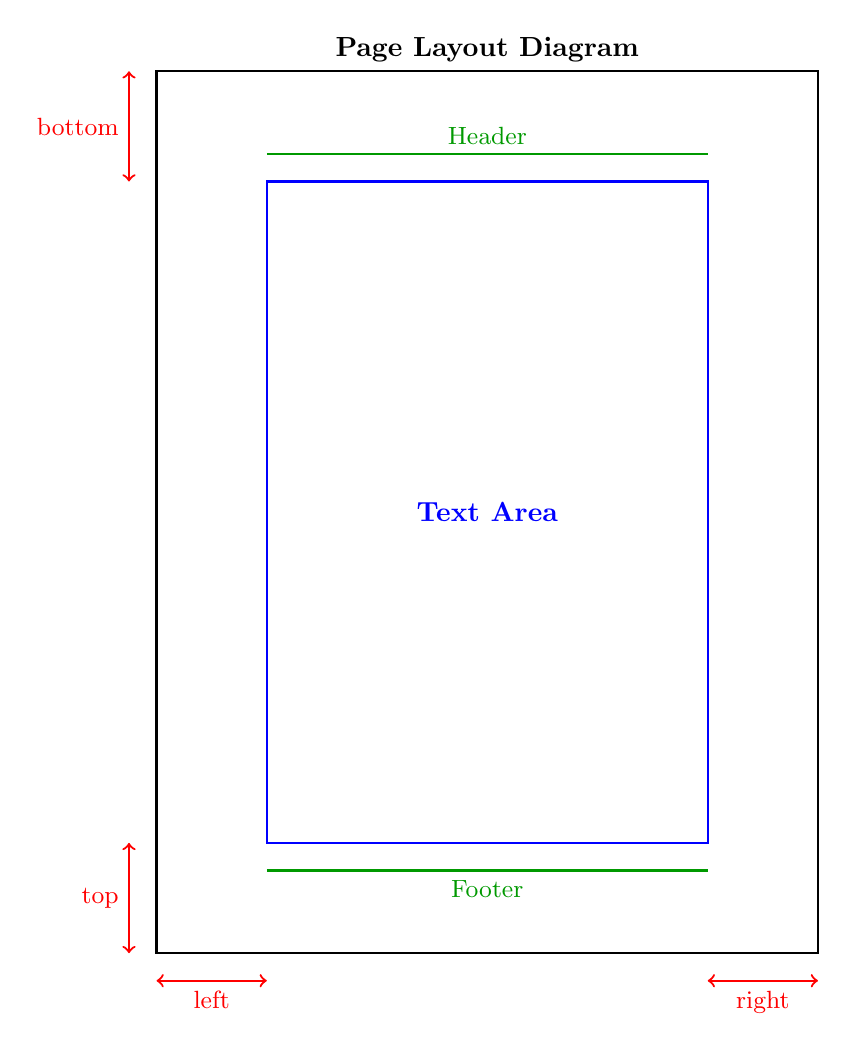
\begin{tikzpicture}[scale=0.7]
    % Page outline
    \draw[thick] (0,0) rectangle (12,16);
    \node[above] at (6,16) {\textbf{Page Layout Diagram}};

    % Text area
    \draw[blue, thick] (2,2) rectangle (10,14);
    \node[blue] at (6,8) {\textbf{Text Area}};

    % Margin labels
    \draw[<->, red, thick] (0,-0.5) -- (2,-0.5) node[midway, below] {\small left};
    \draw[<->, red, thick] (10,-0.5) -- (12,-0.5) node[midway, below] {\small right};
    \draw[<->, red, thick] (-0.5,0) -- (-0.5,2) node[midway, left] {\small top};
    \draw[<->, red, thick] (-0.5,14) -- (-0.5,16) node[midway, left] {\small bottom};

    % Header
    \draw[green!60!black, thick] (2,14.5) -- (10,14.5);
    \node[green!60!black, above] at (6,14.5) {\small Header};

    % Footer
    \draw[green!60!black, thick] (2,1.5) -- (10,1.5);
    \node[green!60!black, below] at (6,1.5) {\small Footer};
\end{tikzpicture}
\caption{Page layout anatomy}
\label{fig:pagelayout}
\end{figure}

% ------------------------------------------------------------------
\section{Headers and Footers (fancyhdr)}

\begin{lstlisting}[language={[LaTeX]TeX}, caption=fancyhdr package]
\usepackage{fancyhdr}
\pagestyle{fancy}

% Clear all defaults:
\fancyhf{}

% Set header:
\fancyhead[L]{Left header}       % L = Left
\fancyhead[C]{Center header}     % C = Center
\fancyhead[R]{Right header}      % R = Right

% Set footer:
\fancyfoot[L]{Author Name}
\fancyfoot[C]{\thepage}          % Page number
\fancyfoot[R]{\today}

% For even/odd pages (twoside):
\fancyhead[LE,RO]{\thepage}      % Left Even, Right Odd
\fancyhead[RE,LO]{\leftmark}     % Right Even, Left Odd

% Rule thickness:
\renewcommand{\headrulewidth}{0.4pt}
\renewcommand{\footrulewidth}{0pt}  % No footer rule

% Chapter page style (plain):
\fancypagestyle{plain}{
    \fancyhf{}
    \fancyfoot[C]{\thepage}
    \renewcommand{\headrulewidth}{0pt}
}
\end{lstlisting}

\subsection{Position Codes}

\begin{table}[H]
\centering
\begin{tabular}{ll}
\toprule
\textbf{Code} & \textbf{Position} \\
\midrule
\texttt{L} & Left \\
\texttt{C} & Center \\
\texttt{R} & Right \\
\texttt{E} & Even page \\
\texttt{O} & Odd page \\
\texttt{LE} & Left on even page \\
\texttt{RO} & Right on odd page \\
\bottomrule
\end{tabular}
\caption{Header/footer position codes}
\end{table}

% ------------------------------------------------------------------
\section{Page Numbering}

\begin{lstlisting}[language={[LaTeX]TeX}, caption=Page numbering]
% Numbering styles:
\pagenumbering{arabic}   % 1, 2, 3 (default)
\pagenumbering{roman}    % i, ii, iii
\pagenumbering{Roman}    % I, II, III
\pagenumbering{alph}     % a, b, c
\pagenumbering{Alph}     % A, B, C

% Set page counter:
\setcounter{page}{1}     % Start counting from 1

% No page number on current page:
\thispagestyle{empty}
\end{lstlisting}

% ------------------------------------------------------------------
\section{Multiple Columns}

\begin{lstlisting}[language={[LaTeX]TeX}, caption=Multiple columns]
% Document-wide twocolumn option:
\documentclass[twocolumn]{article}

% Switch mid-document:
\onecolumn   % Switch to one column
\twocolumn   % Switch to two columns

% With multicol package (more flexible):
\usepackage{multicol}

\begin{multicols}{3}  % 3 columns
    Text in column one continues into
    column two and then column three.
\end{multicols}

\begin{multicols}{2}[Section Title]
    Two-column section with a title.
\end{multicols}
\end{lstlisting}

% ------------------------------------------------------------------
\section{Page Breaks}

\begin{lstlisting}[language={[LaTeX]TeX}, caption=Page breaks]
\newpage         % Start a new page
\clearpage       % Flush all floats, then new page
\cleardoublepage % For twoside: go to next odd-numbered page
\pagebreak       % Suggest a page break (stretchable)
\nopagebreak     % Suggest no page break
\linebreak       % Suggest a line break
\nolinebreak     % Suggest no line break
\end{lstlisting}

% ------------------------------------------------------------------
\section{Paragraph Control}

\begin{lstlisting}[language={[LaTeX]TeX}, caption=Paragraph control]
% Paragraph indent:
\setlength{\parindent}{1cm}         % Set indent width
\noindent                           % No indent for this paragraph
\indent                             % Force indent

% Paragraph skip (no indent, vertical space instead):
\usepackage{parskip}               % Removes indent, adds space

% Or manually:
\setlength{\parindent}{0pt}
\setlength{\parskip}{6pt plus 2pt minus 1pt}
\end{lstlisting}
